\documentclass{article}

\usepackage[utf8]{inputenc}
\usepackage[T1]{fontenc}
\usepackage{times}
\usepackage[margin=3cm]{geometry}
\usepackage{enumitem}

% German
%\usepackage[ngerman]{babel}
% English
\usepackage[english]{babel}

\usepackage[round,authoryear]{natbib}
\usepackage{amsmath,amssymb,amsthm}
\usepackage[hyphens]{url}
\usepackage{caption} 
\usepackage{booktabs}
\usepackage{hyperref}
\usepackage{graphicx}
\usepackage{lipsum}

\graphicspath{ {./images} }
\hypersetup{
    colorlinks=true,
    linkcolor=blue,
    filecolor=magenta,      
    urlcolor=blue,
}
\setlist{noitemsep}

% German
%\newtheorem{definition}{Definition}
%\newtheorem{satz}{Satz}
% English
\newtheorem{definition}{Definition}
\newtheorem{theorem}{Theorem}

% TODO
\author{Alexander Lutsch\\Ephraim Siegfried\\Felix Andrist}
\title{ \Huge Cuisinventory }
\date{Fall Semester, 2023 \\ Computer Architecture}


\begin{document}
\maketitle

\section{Introduction}
\href{https://github.com/EphraimSiegfried/cuisinventory}{Cuisinventory} serves as an intuitive grocery inventory management tool, simplifying the tracking of food consumption and detailed product specifics. This system is embodied in a station equipped with a barcode scanner and a weight scale for interactive use. By scanning the barcode of grocery items at the station, Cuisinventory promptly retrieves pertinent details such as product name, brand, allergens, and storage guidelines. The integrated weighing feature allows for the measurement of grocery weight, and when combined with the system's data on product quantity, Cuisinventory accurately calculates the remaining food quantity as a percentage. All inventory data is stored in a bespoke database and can be conveniently accessed and managed through a dedicated web application that communicates seamlessly with the station.

\section{User Manual}

\subsection{System Overview}
The Cuisinventory system is equipped with an LCD interface and three tactile buttons:
\begin{itemize}
	\item GB1 (Green Button 1): Located above and to the left of the LCD screen.
	\item GB2 (Green Button 2): Positioned below and to the left of the LCD screen.
	\item RB (Red Button): Situated to the right of the LCD screen.
\end{itemize}

\subsection{Initial setup}

\subsubsection{USB-Mode Configuration}
\begin{enumerate}
	\item Connect the system to your computer using a USB cable.
	\item Press and hold RB to enter USB-Mode.
	\item On your computer, locate and open the SD-Storage of the system.
	\item Edit the \textit{settings.json} file to input your Wi-Fi details:
	      \begin{itemize}
		      \item "SSID": Your Wi-Fi network name.
		      \item "PASSWORD": Your Wi-Fi password.
	      \end{itemize}
	\item Save the file and disconnect the USB cable.
\end{enumerate}

\subsubsection{System Registration}
\begin{enumerate}
	\item Locate the system ID beneath the device.
	\item Visit \url{https://ephraimsiegfried.github.io/cuisinventory-web/}.
	\item Log in using your system ID to access and manage your kitchen inventory online.
\end{enumerate}

\subsection{Daily Operations}
\subsubsection{Adding new Products}
\begin{enumerate}
	\item Short press GB1 to initiate the addition process.
	\item Position the product barcode facing downwards and scan it.
	\item Place the product on the Cuisinventory scale.
	\item Confirm to weigh by pressing GB1.
	\item A success message indicates the product has been added successfully.
\end{enumerate}

\subsubsection{Updating new products}
\begin{enumerate}
	\item Short press GB2 to start the update process.
	\item Repeat the scanning and weighing process as described in the addition of new products.
	\item A success message confirms the product weight has been updated.
\end{enumerate}

\subsubsection{Removing Products}
\begin{enumerate}
	\item Short press RB to initiate removal.
	\item Scan the product barcode.
	\item A success message confirms the product has been removed.
\end{enumerate}

\subsubsection{Inspecting Products on the System LCD}
\begin{enumerate}
	\item Long press GB1 to view products.
	\item Navigate through products:
	      \begin{itemize}
		      \item Next product: Short press GB1.
		      \item Previous product: Short press GB2.
	      \end{itemize}
	\item Exit the view by long pressing RB.
\end{enumerate}

\subsubsection{Inspecting Products on the Cuisinventory Website}
\begin{enumerate}
	\item Visit \url{https://ephraimsiegfried.github.io/cuisinventory-web/} to view your entire inventory.
	\item Products can be sorted by date or quantity for easier management.
\end{enumerate}

\subsubsection{Note: Aborting}
For any operation, you can abort and return to the main screen by long pressing RB.

\newpage

\section{Materials and Software}
\subsection{Hardware}
The following table lists the hardware used to implement the project.
\\[10pt]

\begin{tabular}{l l}
	\hline
	Component              & Model                                           \\
	\hline
	Main Controller        & Adafruit Feather nRF52840                       \\
	Barcode-Code Scanner   & SparkFun 2D Barcode Scanner Breakout            \\
	Strain Gauge Load Cell & Strain Gauge Load Cell - 4 Wires - 5Kg          \\
	ADC-Chip               & Adafruit NAU7802 24-Bit ADC - STEMMA QT / Qwiic \\
	Display                & SparkFun LCD-16398                              \\
	WLAN Co-Processor      & Adafruit AirLift FeatherWing ESP32              \\
	I2C Interface          & SparkFun Qwiic / Stemma QT FeatherWing          \\
	3 * Buttons            & SparkFun Zubehör Qwiic Button - Green LED       \\
	Cable                  & SparkFun Qwiic Cable Kit                        \\
	Adalogger              & Adalogger FeatherWing - RTC + SD Add-on         \\
	Stacking Headers       & Adafruit 12-pin and 16-pin female headers       \\
	\hline
\end{tabular} \\[10pt]

Fundamentally, we have the main controller, the Adafruit Feather nRF52840, offering a 64MHz ARM Cortex M4F processor along with 256KB of SRAM.
It supports Arduino libraries and has a wide array of external ports to which we can connect the other components.
We expand the capabilities of our main controller with a WLAN Chip and a SD card.
For the interaction with the controller we use three main buttons, a strain gauge load cell which measures weight, and a barcode scanner.
A small LCD display outputs information.

\subsection{Required Libraries}
Fortunately, each piece of hardware we utilized came with at least one compatible library that facilitated our software development. The table provided below lists the hardware components along with the respective libraries we selected for integration.
\\[10pt]

\begin{tabular}{l l}
	\hline
	Component             & Library                                                                                                         \\
	\hline
	Barcode-Scanner       & \href{https://github.com/sparkfun/SparkFun_DE2120_Arduino_Library}{SparkFun DE2120 Arduino Library}             \\
	Load Cell \& ADC-Chip & \href{https://github.com/adafruit/Adafruit_NAU7802}{Adafruit NAU7802}                                           \\
	Display               & \href{https://github.com/sparkfun/SparkFun_SerLCD_Arduino_Library}{SparkFun SerLCD Arduino Library}             \\
	WLAN Co-Processor     & \href{https://github.com/adafruit/WiFiNINA}{WiFiNINA Adafruit Fork}                                             \\
	Buttons               & \href{https://github.com/sparkfun/SparkFun_Qwiic_Button_Arduino_Library}{SparkFun Qwiic Button Arduino Library} \\
	Adalogger             & \href{https://github.com/adafruit/SdFat}{SdFat Adafruit Fork}                                                   \\
	\hline
\end{tabular} \\[10pt]

Additionally, we also utilize the SPI, Wire, and SoftwareSerial libraries included in the Arduino Core, which facilitate communication protocols via the designated pins on our main controller.

On the software side, we employ the \href{https://github.com/arduino-libraries/ArduinoHttpClient}{Arduino HTTP Client} library, enhancing our ability to structure and manage the sending and receiving of HTTP requests.

A critical library for this project is the \href{https://github.com/bblanchon/ArduinoJson}{Arduino Json Library}, which plays a vital role in the correct serialization and deserialization of JSON files on our local controller and SD card. Our database logic is fundamentally dependent on the efficient handling of data in JSON format.

\subsection{Software Development}
For our coding collaboration, we employed git version control in conjunction with GitHub. Initially, we used the Arduino IDE but soon found its capabilities lacking for our needs. This led us to transition to PlatformIO, which offered a more professional development environment. PlatformIO's features, such as the ability to define various environments for compilation and its automated library management through a centralized configuration file, significantly enhanced our workflow.

With PlatformIO, we enjoyed the flexibility of coding in our preferred editors and not being constrained by file naming rules like the .ino extension. Moreover, it facilitated the easy integration of unit tests for our critical classes.

We also leveraged the synergy between GitHub and PlatformIO to establish a continuous integration system. This system utilizes GitHub Actions for code style formatting and code compilation. Furthermore, PlatformIO's remote execution function allowed us to perform unit tests on the controller directly through GitHub Actions, adding another layer of efficiency and rigor to our development process.

\section{Implementation}

\subsection{Hardware}

\subsubsection{Putting the sensors together}
Our project involves numerous hardware components, and it was crucial to ensure their compatibility with the microcontroller. The initial step involved integrating the SD Card extension (Adalogger) and the WLAN Co-Processor. These components, roughly the same size as the microcontroller, were conveniently stacked using stacking headers directly atop the main controller.

\begin{figure}[h]
	\centering
	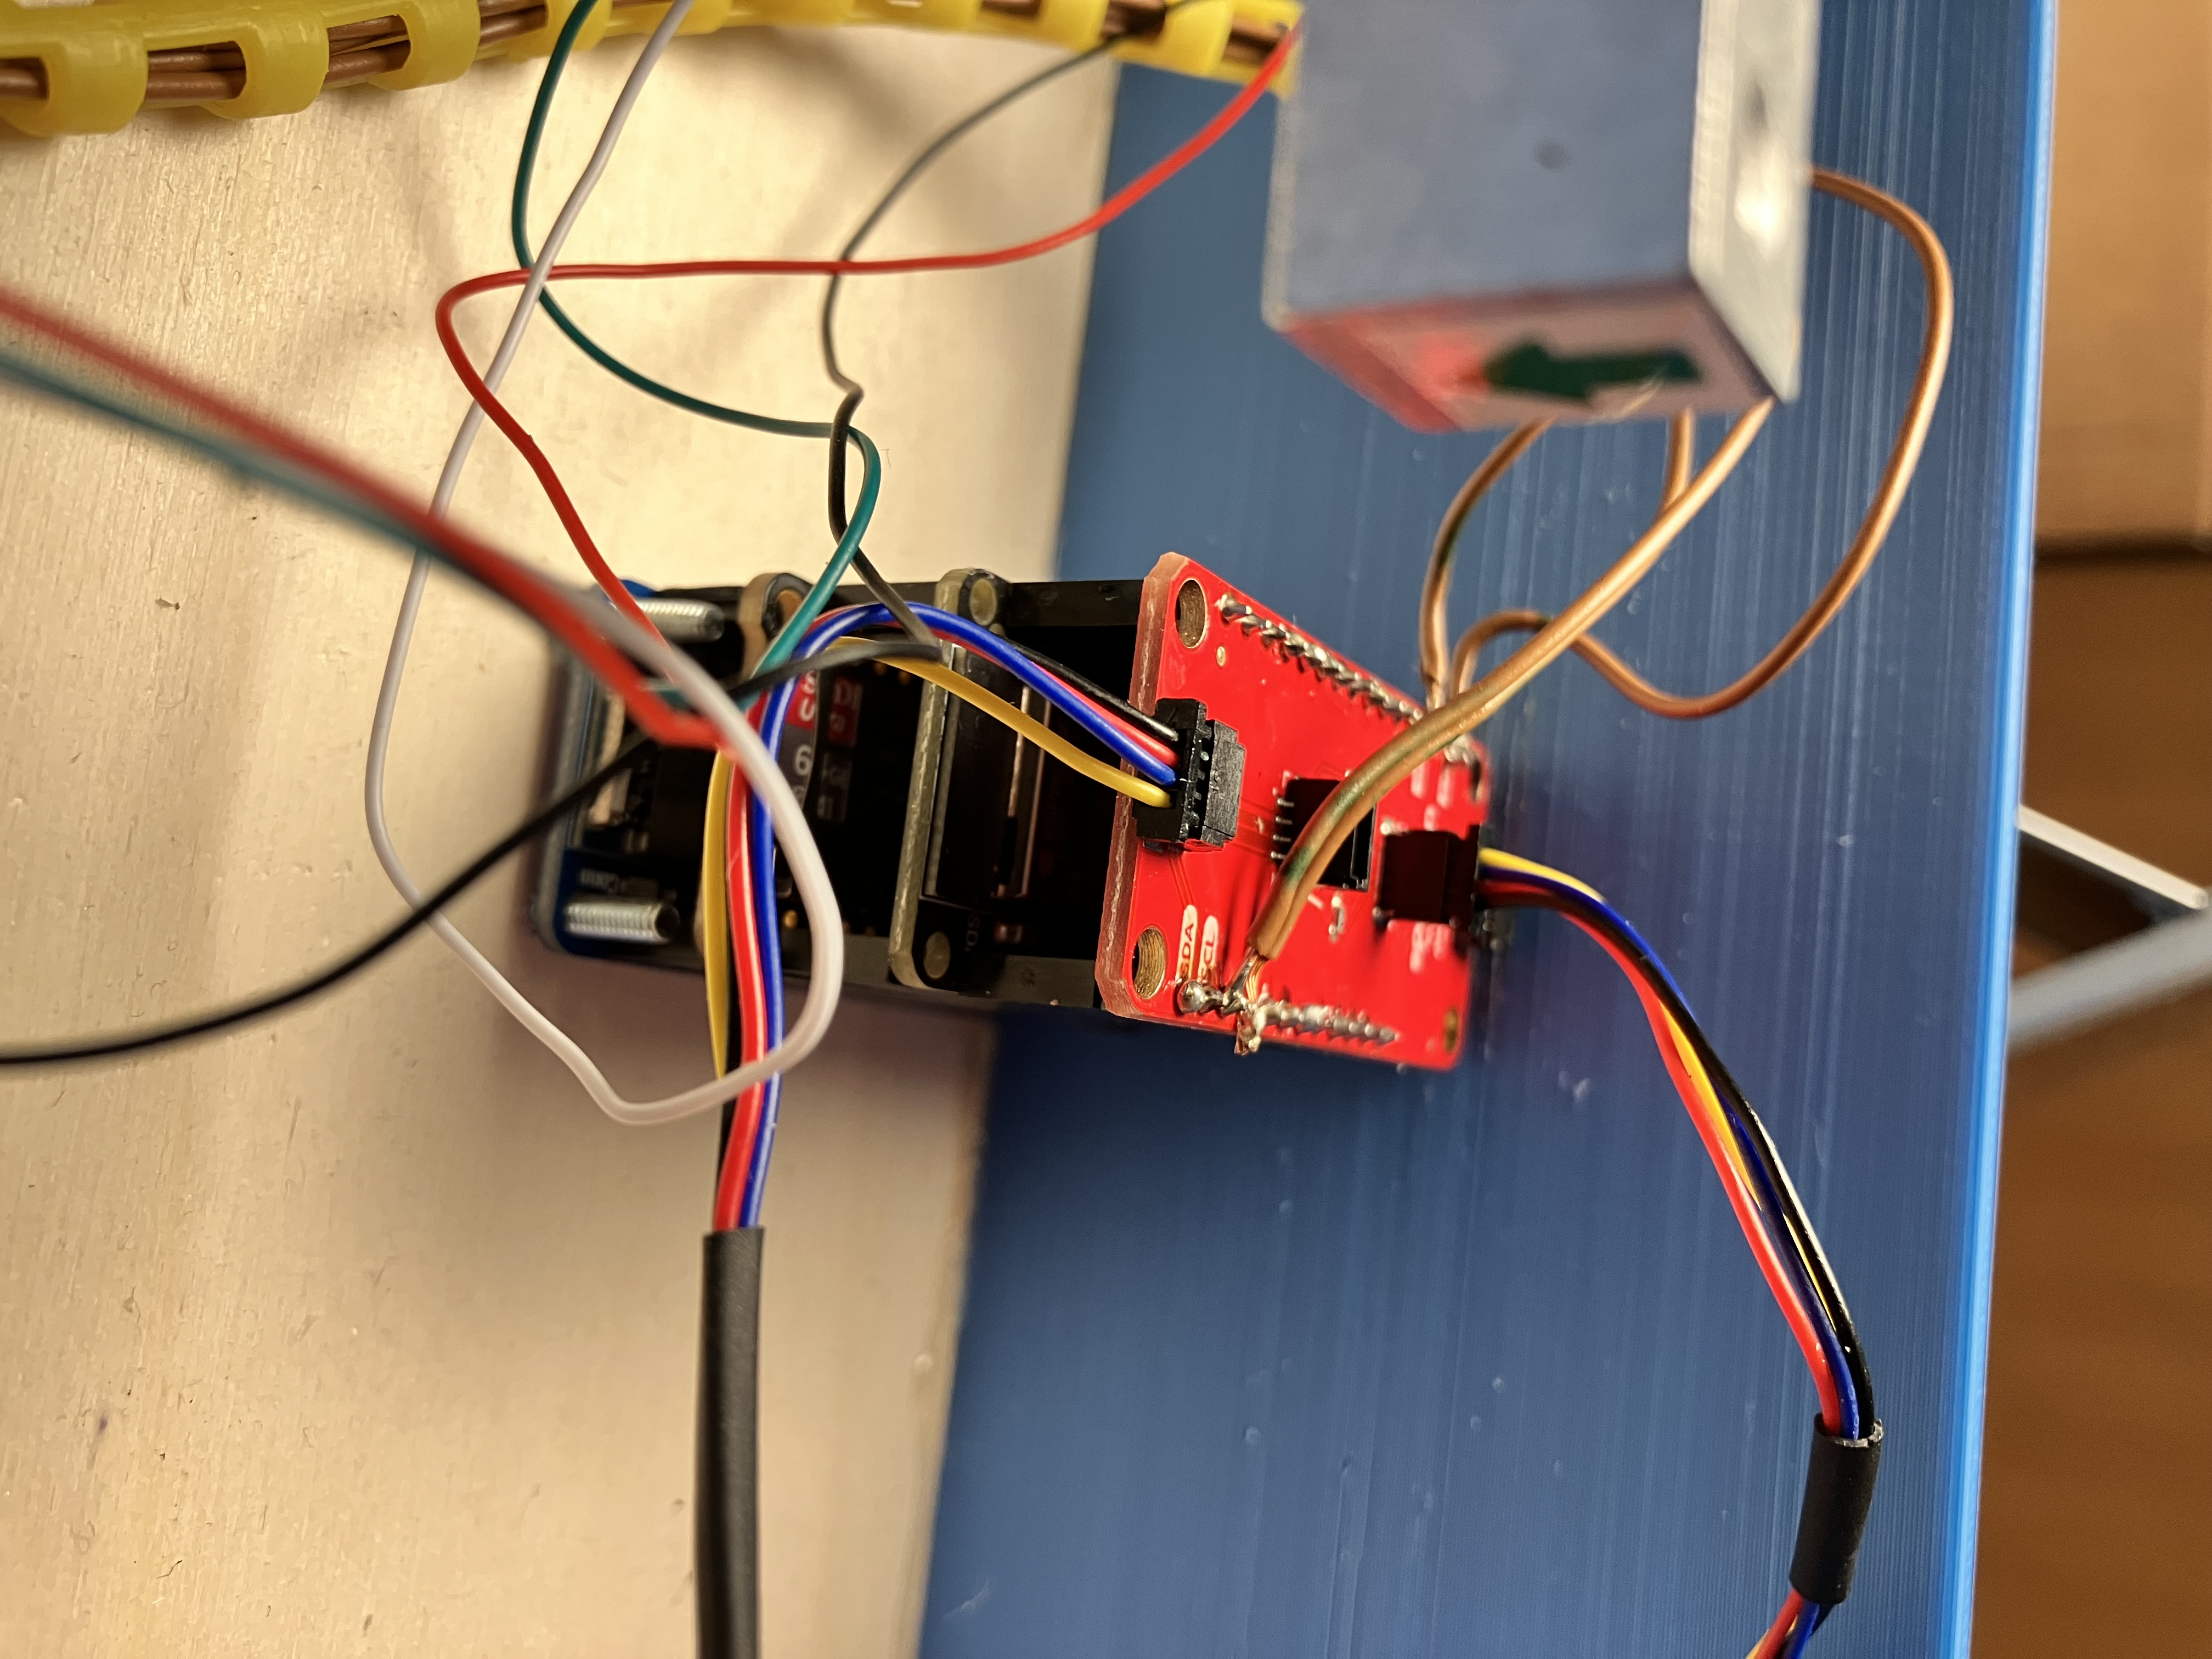
\includegraphics[angle=90,width=0.3\textwidth]{controller.jpeg}
	\caption{Stacking Wifi and SD Card}
	\label{fig:mesh1}
\end{figure}

The remaining components include the strain load cell, the ADC chip for weight measurement, an LCD, three buttons, and a barcode scanner. All of these, except the barcode scanner, communicate via the I2C protocol, which is beneficial since it allows multiple devices to share the same bus.

The three buttons, the ADC weight chip, and the LCD were all connected to the same I2C bus. We utilized the SparkFun Qwiic I2C connectors, which facilitate connections through a daisy chain system, significantly reducing the need for soldering. The QWIIC connectors necessitated a SparkFun Qwiic Shield board, which provides four Qwiic connector ports. This shield board was then connected to the I2C pins of the main controller, with additional stacking pins above the other components.

The final component, the Barcode Scanner, employs UART for communication and was connected to the available RX and TX pins. With all components connected, our last step was to ensure no I2C address conflicts among the devices on the single I2C Bus. We resolved potential conflicts by manually altering the I2C addresses of the three buttons using their software library.

\subsubsection{Building the case}
We wanted to build a case that houses all required hardware components and offers convenient interaction with them in the scope of a kitchen station inventory management system.
\subsection{Software}
The Cuisinventory station fundamentally has five functions that are offered to the user. The first three are managing the inventory: Adding a product, updating the weight of a product and removing a product.
The last two are displaying the inventory on the local LCD and putting the main controller in USB mode, such that the user can make changes to the configuration files on the local SD card.
These functions are coded in the main logic with calls to secondary classes which contain the implementation for necessary hardware and software components.
Additionally, the main logic contains the necessary initializations for the hardware components.
\subsubsection{Buttons}
For the Buttons we rely on the \href{https://github.com/sparkfun/SparkFun_Qwiic_Button_Arduino_Library}{SparkFun Qwiic Button Arduino Library} with which we can read out the buffer of presses, which are saved on the button itself.
We wrote the logic for reading the input of a desired button and filtering out input from the buffer that happened too long ago.
Additionally, we can differentiate between a long and a short press of the button, as "button down" and "button up" are separate events with their own timestamp.

\subsubsection{LCD Display}
The LCD, operated through the \href{https://github.com/sparkfun/SparkFun_SerLCD_Arduino_Library}{SparkFun SerLCD Arduino Library}, is straightforward to utilize. It is directly initialized in the main logic and employed within the primary functions to display information to the user.

\subsubsection{Scale}
The weight sensor consists of two parts: the strain load cell, which sends electrical output based on the strain it's put on, and the analog to digital converter (ADC chip) which interprets this output into a digital value.
For the ADC chip, we rely on the \href{https://github.com/adafruit/Adafruit_NAU7802}{Adafruit NAU7802} library to read digital measurements.
These measurements then have to be converted to grams by multiplication with a factor.
The ADC chip has its own module file, in which we handle initialization and calibrating the offset at the start to zero.

\subsubsection{Barcode Scanner}
The barcode scanner is the only sensor connected over UART. It contains an internal buffer with successfully read barcodes.
We use the \href{https://github.com/sparkfun/SparkFun_DE2120_Arduino_Library}{SparkFun DE2120 Arduino Library} to interact with the scanner.
The usage is pretty straightforward, we basically have to initialize the sensor, and we can then read out the internal buffer.

\subsubsection{Wi-FI Service}
For the WLAN Co-Processor, we rely on the \href{https://github.com/adafruit/WiFiNINA}{WiFiNINA Adafruit Fork} library.
The logic concerning WLAN initialization and internet communication is found in an own class named WIFIService.

When initializing, we try to connect to a Wi-Fi network using the SSID and password, which are found on a JSON file saved on the SD card.
After the user scans a barcode, we have to fetch information from an external barcode database. In our case, the barcode API from https://world.openfoodfacts.org/ is free and offers an excellent amount of information about a wide range of products.

Our WIFIService class handles sending a http request to the API with the help of \href{https://github.com/arduino-libraries/ArduinoHttpClient}{Arduino HTTP Client}.
The response will be a JSON containing the information, which is processed with the \href{https://github.com/bblanchon/ArduinoJson}{Arduino Json Library}. Furthermore, the WIFIService class is also responsible for transmitting inventory data to our server hosted on \href{https://www.pythonanywhere.com/}[Pythonanywhere server]. This server is integral to our system, processing requests from both the web client and the kitchen system. It enables users to view their inventory on the cuisinventory website, ensuring a seamless integration between the client interface and the backend inventory management.

\subsubsection{SD card and the Database class}
We have a micro SD card in our "Adalogger" module, on which we want to save our inventory information.
For writing and reading from the SD card, we work with the \href{https://github.com/adafruit/SdFat}{SdFat Adafruit Fork} library.
The logic of the database is found in the "DBClass" class. Fundamentally we want to save all relevant information about the products in the inventory in JSON Files on the SD card.
The DBClass provides methods for saving and retrieving information, it relies heavily on the \href{https://github.com/bblanchon/ArduinoJson}{Arduino Json Library} with which we serialize and deserialize JSON files.
As we have to work with the limited amount of RAM on a microchip, we can't just put the entire inventory in a single JSON file.
Instead, every product in the inventory has its own JSON File and we generate unique IDs to differentiate them. We have to do this as our inventory can contain multiple products with the same barcode.
These unique IDs are written into the JSON file of the product, and the JSON file itself has the unique ID as filename when saved on the SD card.
To work with all the JSON files, we keep two mapping files on the SD card. One mapping file contains every unique ID and its corresponding barcode.
The other mapping file contains every barcode and a list of corresponding unique IDs. The mapping files are also saved as JSON Files.
These two mappings enable us to quickly find the corresponding files when searching for a barcode and also contain an overview of all products in the inventory.

\subsection{Pythonanywhere Server and Webclient}
For an engaging and user-friendly interface to view the digital inventory, we opted to develop a web client. The cuisinventory website allows users to view all products, organize them, and access detailed information, including nutritional facts. The webserver is implemented using a stack comprising Javascript, React, Vite, Tailwind, and DaisyUI.

The web client maintains communication with our Pythonanywhere server, which serves as a central hub, processing requests from both the web client and the kitchen system, and managing the complete inventory database. The kitchen system interacts with the Pythonanywhere server to update inventory data using PUT requests, while the web client retrieves this information through GET requests. The Pythonanywhere server is built using Python and the Flask framework.

\section{Problems and Solutions}

\subsection{Arduino IDE Troubles}
When starting out on the project we produced our first few lines of code using Arduino IDE, however as the project became bigger we ran into several inconveniences.
Arduino IDE fundamentally puts everything into a single .ino file for compilation. With additional .cpp files used for code structure there is an annoying limitation that it still requires a .ino file with the parent folder name being the same as the .ino file.

As we have a lot of hardware and an adafruit controller, we needed to install specific Adafruit library forks for the code to run.
Since Arduino IDE doesn't offer collaborative library management, you had to make sure to have the correct libraries and library versions set up correctly on every single client.

When we finished work on a relevant module like the database class, Arduino IDE provided no testing framework for unittests which we could easily use to ensure correctness.

Lastly, we also wanted to use external code editors instead of working with the Arduino IDE interface.
We did some research into alternatives and pleasantly found PlatformIO, an IDE for embedded software development.
It very much offered all we were looking for; we can define our platform, the specific microcontroller, and then list all required libraries and versions in a single central configuration file.
With the "Unity" test framework, we also set up unit tests for our Wi-Fi and database functions.
Now running or testing the project just requires to pull it from GitHub and run it with PlatformIO.

\subsection{Database}
When programming the database logic, which was supposed to hold information about the inventory, we struggled with the RAM constrains of a microcontroller.
We looked into SQL but soon found that a SQL database on a microcontroller doesn't make sense as you run into processing power and RAM limitations.
We then settled for the JSON format, which seemed like a solid way to store information and there was an Arduino JSON library available.
However we couldn't just store all products in a single inventory JSON file, as eventually opening this file would fill up our available RAM.
So we came up with the idea to simply store single JSON files for each product and, in additional files, store logical mappings so we are able to find the relevant files again.
Getting this to work correctly took a lot of unit testing, as saving the files correctly on the SD card and editing the mappings with the Arduino JSON library was prone to errors.

\subsection{SD Card Library}
We initially used the standard \href{https://github.com/arduino-libraries/SD}{Arduino SD Library} for writing and reading files on the SD card. The bulk of our database logic was implemented using it.
It had annoying limitations, like the filename not being allowed to be over 8 characters, but that was acceptable.
However as we began to use folder structures for saving files, we also found out that the library doesn't support deleting a folder containing other files, even though the documentation states that the folder deletion works recursively.
This was a problem, especially for testing, so we started looking for alternatives. We found that the SD library is in reality a simple wrapper for the more powerful \href{https://github.com/greiman/SdFat}{SD Fat} library, which offers more functions and fewer limitations.
And luckily we also found an \href{https://github.com/adafruit/SdFat}{SdFat Adafruit Fork} for our microcontroller. Fearing that with the new library we would need to rewrite a lot of the implementation, we switched to it.
To our surprise, we didn't need to change a single line of code in our database logic for it to work. It used the same class and function names as before, only now we had access to more useful functions like recursively deleting directories.
This was a funny exception for us, as so far, things generally didn't work when trying them out.

\section{Summary}
At the beginning of the planning phase, we were looking for a project idea that offered enough complexity, while also being something that we would consider useful.
With Cuisinventory, a grocery inventory management system, we found such an idea. The amount of hardware components and software logic we needed to implement the functionality fulfilled our complexity requirements.
Furthermore, we also implemented an external web server and the whole station had a case we designed and built using 3D printing and woodworking.
To achieve all this, we needed regularly scheduled meetups on which we worked together and set goals for the implementation of components and logic.
In this project we also set up more efficient collaboration processes, like switching to a more convenient integretion  and implementing automated GitHub actions.
As we managed to actually implement all of this without cutting corners, we are happy with the result of the project.
However we also encountered bugs which were not reproducable with unit tests, for example the microcontroller failing to concatenate strings correctly and constant Strings being overwritten.
Furthermore some of the QWIIC connector I2C cables in use also showed loose contacts.
These issues lead to bugs that are difficult to reproduce and would require additional work to completely iron out.

\section{Links}

\begin{description}
	\item [Kitchen Station Repository]\url{https://github.com/EphraimSiegfried/cuisinventory}
	\item[Web Client Repository] \url{https://github.com/EphraimSiegfried/cuisinventory-web}
\end{description}



\end{document}
